\section{Problem Formulation}\label{sec:problem}

\subsection{Conditional causal usefulness}\label{sec:conditional-usefulness}

Let $f$ be a transformer evaluated by a scalar task metric $m$. We consider two executions of the same task instance: an intact state $A$ and a perturbed state $B$, where $B$ is produced by a prespecified intervention on a primary circuit component or set of components. Let $h$ denote a candidate attention head whose change in functional importance we want to explain.

For context $s\in\{A,B\}$, let $m_s^{h}$ be the task metric with $h$ operating normally and $m_s^{0}$ the metric when $h$ is zeroed while the rest of context $s$ is held fixed. We define the candidate's output-grounded causal usefulness as
\begin{equation}
E_s(h)=m_s^{h}-m_s^{0}.
\label{eq:context-effect}
\end{equation}
The cross-state change to be explained is
\begin{equation}
\Delta_h=E_B(h)-E_A(h).
\label{eq:conditional-gain}
\end{equation}
We call $\Delta_h$ the \emph{conditional gain}. Positive $\Delta_h$ means that the candidate's contribution becomes more positive after the primary intervention; it does not by itself imply that the candidate is helpful in the perturbed state. We use \emph{positive functional recruitment} only when both $E_B(h)>0$ and $\Delta_h>0$.

Because the candidate-present and candidate-zero conditions are compared within the same surrounding context, $\Delta_h$ is not simply the change in task performance from $A$ to $B$. It is the change in the candidate's marginal causal contribution under the specified intervention.

\subsection{Mechanism-resolution objective}\label{sec:mechanism-objective}

FALI begins after a candidate head and a task-relevant target edge or edge set have been specified, for example by prior circuit analysis, conditional co-ablation, patching, or a task-specific hypothesis. It does not search over heads or discover a circuit automatically.

The objective is to account for $\Delta_h$ using changes in three architecture-level objects: the candidate's attention scores, its value vectors, and the surrounding computation in which its output is used. We further partition the score tensor into the task-target score, competing scores in the same query row, and all other structurally valid scores. This yields a controlled mechanism-discrimination problem: under a fixed intervention algebra, which candidate-local or surrounding changes receive credit for the observed change in output-grounded usefulness? Figure~\ref{fig:fali-overview} summarizes the setup.

\begin{figure*}[t]
\centering
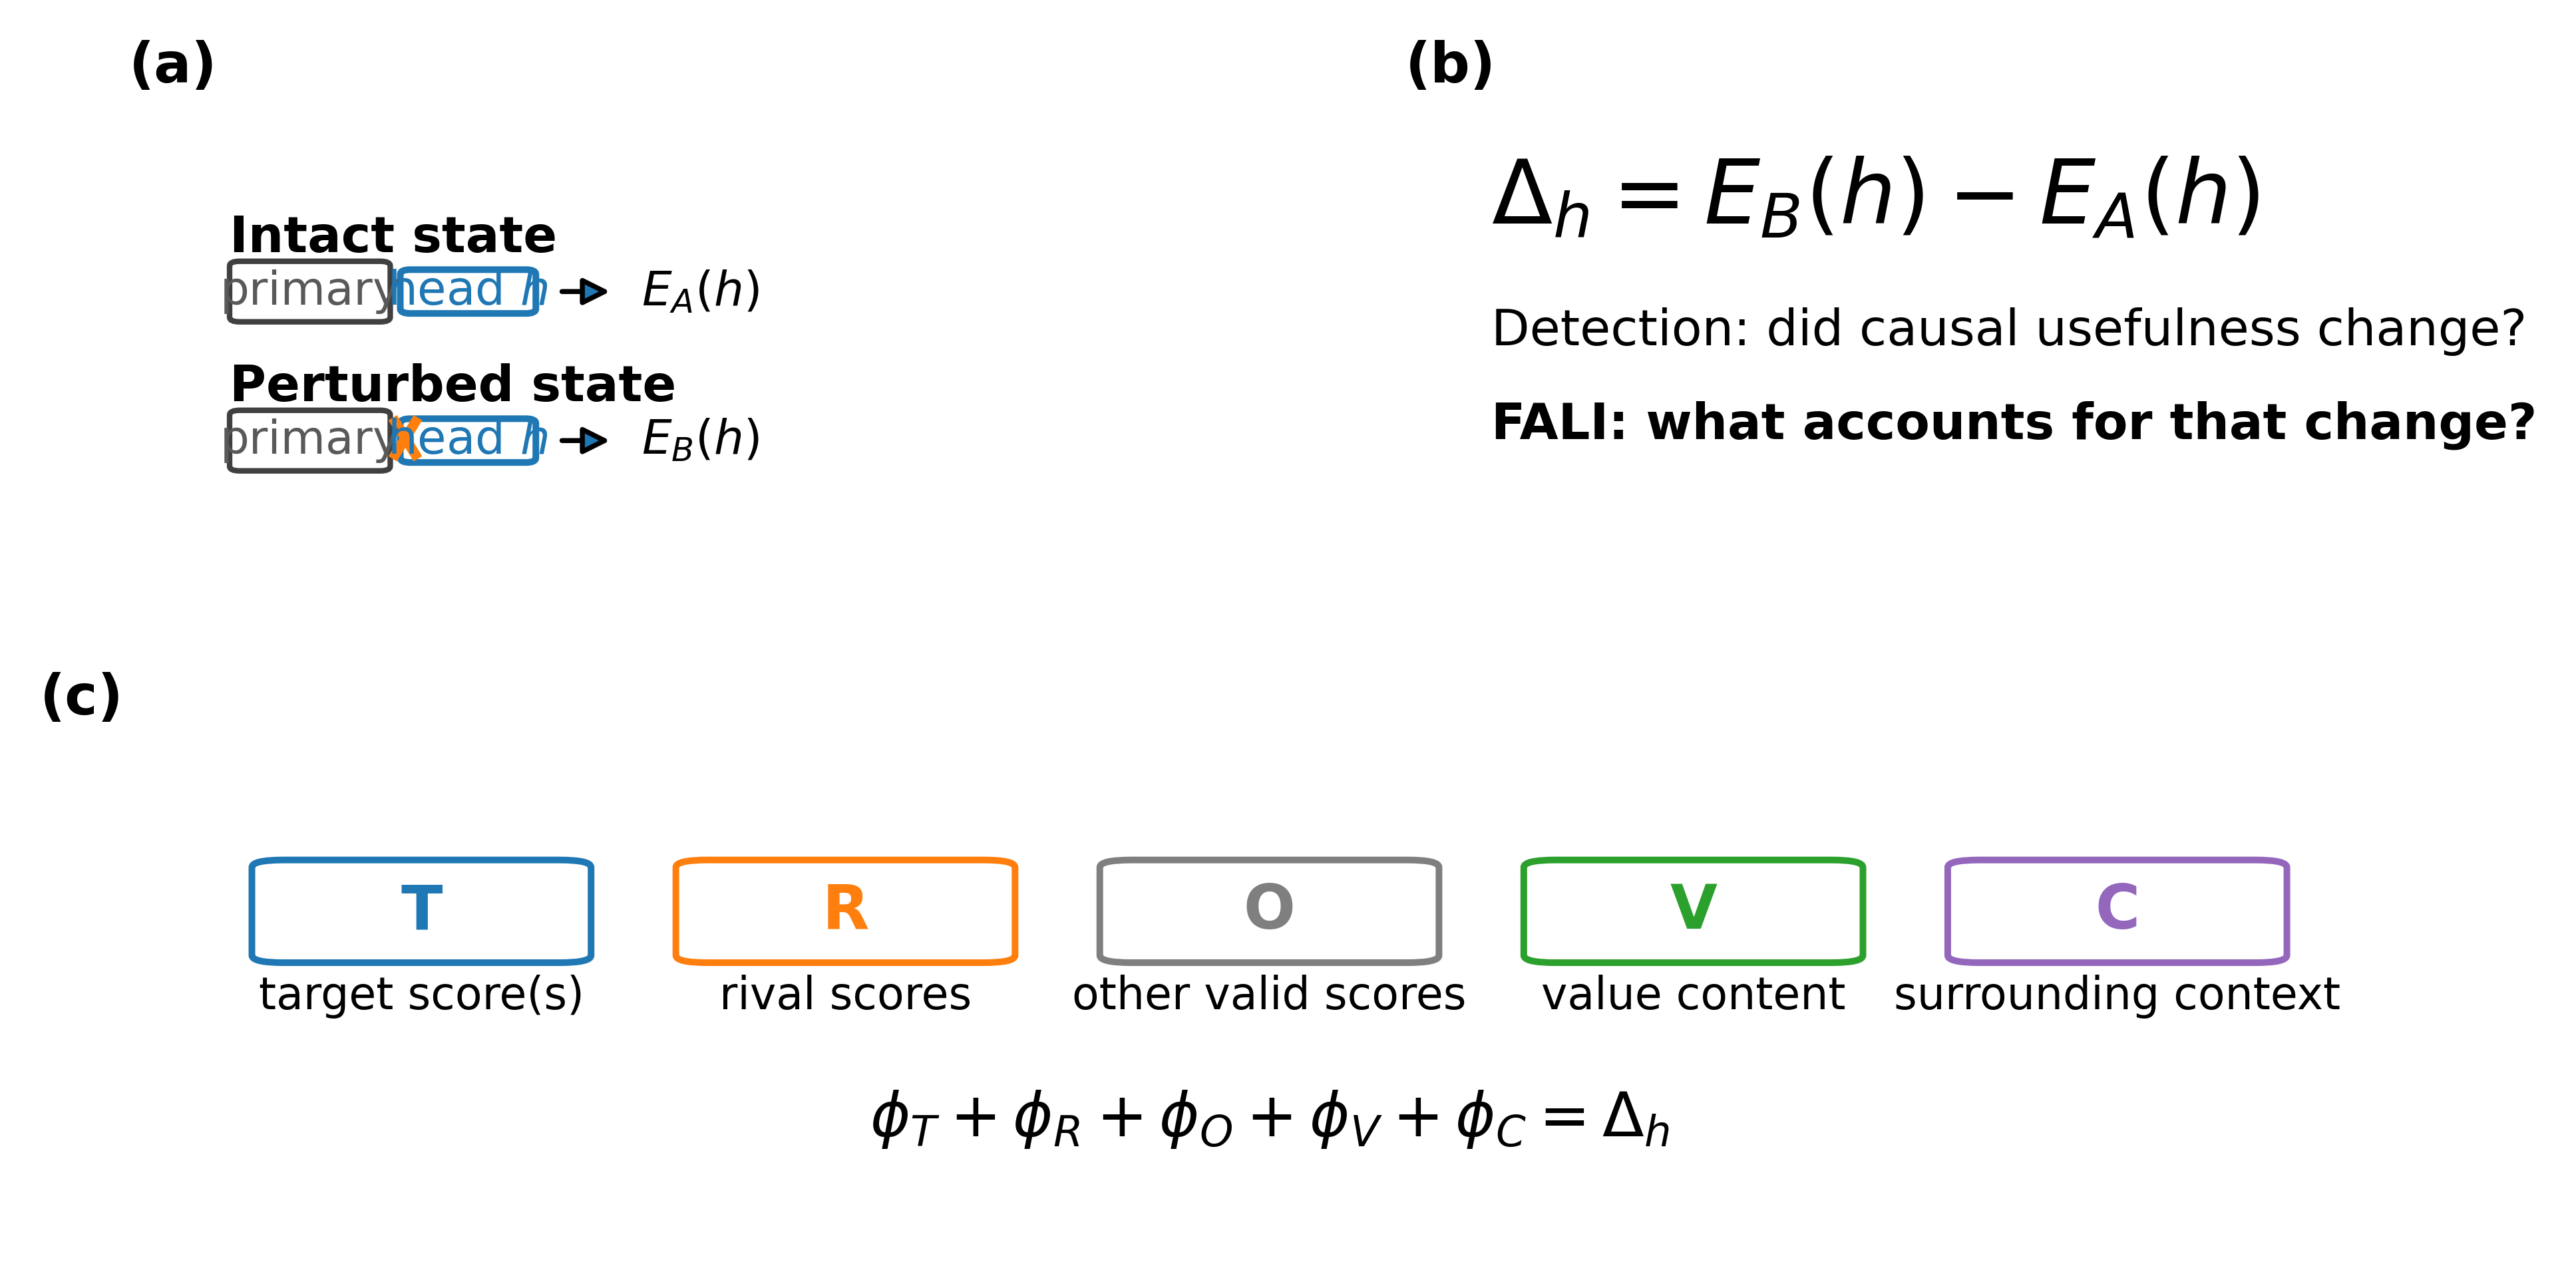
\includegraphics[width=\textwidth]{figures/Fig1.png}
\caption{\textbf{FALI explains a conditional change in candidate-head usefulness.}
The candidate head has output-grounded causal usefulness $E_A(h)$ in the intact context and $E_B(h)$ after the prespecified primary-circuit perturbation, with $\Delta_h=E_B(h)-E_A(h)$ the cross-state change to be explained.
FALI allocates this change among target scores ($T$), rival scores ($R$), other valid scores ($O$), value content ($V$), and surrounding-network context ($C$).
The candidate head and task-relevant target coordinates are specified before FALI analysis; the resulting attributions are defined by the explicit counterfactual intervention game.}
\label{fig:fali-overview}
\end{figure*}

